%!TEX root = main.tex


Causal statistical decision theory offers a different set of basic assumptions to causal reasoning based on causal Bayesian networks, and also offers an identification theorem that applies to situations where the backdoor criterion of CBNs applies, but makes a different set of furhter assumptions to derive this result.

In particular, CSDT avoids the need for a \emph{do-scheme}, an assumption that I find particularly hard to evaluate as I explain below. One of the costs of adopting the CSDT view is the lack of a formal definition of ``causal effect''. Under the right conditions CSDT features stable relationships between random variables that may be informally interpreted as causal effects, but this is only at the level of informal interpretation.

Whether the assumptions underlying CSDT are better than those underlying the CBN for any class of questions is not easy to say. Addressing it, I would imagine, should proceed from adopting an established criteria for judging assumptions and comparing assumptions that differ under each framework according to these criteria. There would be a substantial amount of work involved in doing this and it's not presently in scope.

\subsection{Evaluating Assumptions (philosophy is hard)}

Tentatively, the following properties of assumptions seem desirable:
\begin{enumerate}
	\item People who are solving problems should be able to evaluate assumptions with a low rate of false positives (i.e. problems where further assumptions are judged to hold but in fact they do not)
	\item False negatives should be minimised subject to the requirement of a very low number of false positives (i.e. as long as it doesn't increase the false positive rate, it is desirable to find more problems that can be solved by a particular theorem)
	\item Assumptions and results should exhibit continuity - where an assumption holds approximately, approximate results follow
\end{enumerate}

Knowing how well assumptions satisfy these criteria is usually difficult. For example, we may not have any ground truth answers at all for whether some assumptions hold or not, and so whatever we can say about false positive rates is limited. This raises the possibility of a further desirable property of an assumption: we have some information about how well it satisfies 1-3. This addition invokes a meta-assumption that assumptions with a track record tend to be better than those without.

Actually, these desiderata don't seem quite right. Suppose A1 is an appealing but usually false assumption - i.e. it is subject to a high false positive rate. The desiderate imply that A1 is inferior A1 + F, where F stands for an assumption universally judged to be a contradiction. This violates the common notion that it is always better to work with fewer assumptions (though it does have a degree of plausibility - ``everyone believes A1 is true, but everyone would be better off believing that A1 is false'').

It's not obvious to me whether the CBN or CSDT approach is unequivocally better with regard to the criteria above.

\subsection{The switch and lightbulb}

The two approaches will be compared using the test case of ``the switch and lightbulb''. This is intentionally chosen as a very simple problem of causal inference.

\begin{quote}
	There is a lightbulb and a switch (maybe there are other things as well). We have a set $D$ of actions available, some of which we know turn the switch on and the rest of which we know turn the switch off, but the effect of any action on the lightbulb is uncertain. We have a very large number $N$ of IID observations of the joint state of the lightbulb and switch. We are interested in choosing decisions that control the light.
\end{quote}

This problem exhibits a number of features which we take to be common to any statistical causal decision problem:
\begin{itemize}
	\item There is a set of decisions, known in advance, that may be chosen
	\item We possess some incomplete prior knowledge about the effects of decisions
	\item Data is available (observations of the switch and light state)
	\item The objective is to control some feature of the environment
\end{itemize}

This problem supports many different modes of operation. For example, we might have:
\begin{itemize}
	\item The switch always turns the light on both in observations and as a result of our actions (more precisely, the switch and light always share the same state in observations and for all actions)
	\item In observations the light is on iff the switch is on, some actions preserve this relationship (``just turn the light on'') while some break it (``cut power to the house, turn the light on'')
	\item There is another switch (``switch 2'') in the house which also controls the light which is randomly on or off in observations. Thus in observations the light is uncorrelated with switch 1 but there are nevertheless actions available that control the light: ``turn switch 2 on, then turn switch 1 on''
\end{itemize}

Consider this problem setup with two additional assumptions: (1) the light operates according to the same rules in both observations and interaction and (2) there is only 1 way to switch the light off and 1 way to switch it on (i.e. $|D|=2$). In this case, however we observe the light to behave when the switch is off is how it must behave when we turn the switch off, and similarly how we observe the light to behave when the switch is on must be how it behaves when we turn the switch on as the observed behaviour in each case must be the behaviour of the light under the unique ``off'' and ``on'' actions. Suppose we instead assume (2') there is only 1 way to switch the light off and there are 2 ways to switch it on (let's call them $d_1$ and $d_2$). In this case we can still determine the behaviour of the light from observations when we turn the switch off, but we cannot determine as much about it when we switch it on - the best that we can say is that some mixture of $d_1$ and $d_2$ will reproduce the observed behaviour of the light when the switch is on. This doesn't limit the behaviour of the light under $d_1$ - if we observe the light was on every time the switch was on, but this was always the result of taking $d_2$, then it is perfectly possible that $d_1$ never switches the light on. On the other hand, if we always observe the light is on when the switch is on, then a random action that takes $d_1$ half the time and $d_2$ half the time must leave the light on at least half the time.


\subsubsection{Using Causal Theories}

To model this situation with a causal theory, we need to define the Markov kernel representing the coupled observation model $\mathscr{H}:\Theta\to \Delta(\{0,1\}^2)$ and consequence model $\mathscr{C}:\Theta\times D\to \Delta(\{0,1\}^2)$. The latent space $\Theta$ represents the set of coupled models we consider to be possible.

If we make no assumptions beyond what was specified in the problem, our observatonal model should admit every possible distribution in $\Delta(\{0,1\})^2$. Because we've made not assumptions about how observations go with consequences, each possible observational distribution will go with each possible consequence.

We have assumed that some decisions are known to turn the switch on and some turn the switch off. Let decisions be enumerated with an integer index $j$, and suppose $d_j\in D$ is a decision that turns the switch off iff $j<=0$. That is, we have

\begin{align}
\mathscr{C}_{\RV{S}_c|\RV{D}} = \begin{cases}
d_j \mapsto \delta_1 & j>0\\
d_j \mapsto \delta_0 & j<=0
\end{cases}
\end{align}

The ``post-decision'' state of the light $\RV{L}_c$ conditioned on the switch $\RV{S}_c$ and the decision $\RV{D}$ is given by $\mathscr{C}_{\RV{L}_c|\RV{S}_c\RV{D}}$ and like the observations is unrestricted. 

Thus $\Theta$ must represent the cartesian product of the set of observational distributions $\Delta(\{0,1\}^2)$ and set of possible conditionals $\mathscr{C}_{\RV{L}_c|\RV{S}_c\RV{D}}$. We can represent the latter set as $[0,1]^{2|D|}$ - the distribution of the binary $\RV{L}_c$ can be parametrised by $p\in [0,1]$, and each possible model assigns a particular parameter $p_{d_j}\in [0,1]$ to each $d_j\in \RV{D}$, giving $\Theta = \Delta(\{0,1\}^2)\times [0,1]^{2|D|}$.

This general setup adds to the given information in the problem in that it supposes that the unknown things - namely, what the light will do given the various decisions available to us - should be represented as probability distributions. In addition, we add the assumption that $D$ is countable. Otherwise, we have as far as possible represented just the information given, and we conclude (as we ought to from the original setup) that we do not possess sufficient information to control the light.

Under some assumptions, we may be able to control the light. For example, suppose $|D| = 2$, with one decision that turns the switch off and one that turns it on (decisions may still have side effects, but this rules out the possibility that there may be two decisions that turn the switch off each with \emph{different} side effects). Suppose  also that the problem is \emph{reproducible} - that is, there is some stochastic action $\gamma\in \Delta(\mathcal{D})$ such that $\gamma \mathscr{C}_{\RV{L}_c\RV{S}_c|\RV{D}} = \mathscr{H}_0$. Then it follows that $\mathscr{C}_{\RV{L}_c|\RV{S}_c\RV{D}} = \mathscr{H}_{\RV{L}_o|\RV{S}_o}\otimes \stopper{0.25}_D$ and so the light may be controlled to the extent permitted by $\mathscr{H}_{\RV{L}_o|\RV{S}_o}$. This is a special case of Theorem \ref{th:riid_ident}, and is a formalisation of the informal result above.

If we suppose that there are two decisions that turn the switch on - $d_1$ and $d_2$ - then we can derive inequality constraints on the consequences of mixtures of $d_1$ and $d_2$. Fix a state $\theta^*\in\Theta$ and let $p_{(on)}:= \mathscr{H}^{\theta^*}_{\RV{L}_o|\RV{S}_o}(1;\{1\})$ be the observed probability that the light is on given that the switch is on. Then given the mixed decision $\gamma=a \delta_{d_1} + (1-a)\delta_{d_2}$ and supposing $a>0.5$, we can say that 

\begin{align}
\mathrm{min}(0,p_{(on)}-a) \leq (\gamma\mathscr{C}^{\theta^*})_{\RV{L}_c|\RV{S}_c} \leq \mathrm{max}(1,p_{(on)}+a) \label{eq:three_decisions}
\end{align}


\subsubsection{Using Causal Bayesian Networks}

In order to approach this problem using causal Bayesian networks we must represent our assumptions in a graph $\mathcal{G}$ over some set of variables, and we must furthermore provide a \emph{do-scheme}, which is a map from the set of decisions $D$ provided by the problem. I am not aware of a set of instructions anywhere about how this ought to be done, and as we will see the process of doing so is less straightforward than one might expect.

To begin with, it is very difficult to model this problem with a CBN without adding more assumptions than are necessary to model the problem with a causal theory. If we use causal language informally, we have posited a decision that can influence the state of a switch and a light. If we propose causal random variables $\RV{D}$, $\RV{S}$ and $\RV{L}$, then we might turn this sentence into the following diagram:

\begin{align}
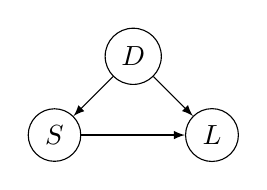
\begin{tikzpicture}[-latex]
\path (0,0) node[draw,circle] (D) {$\RV{D}$}
++(-1,-1) node[draw,circle] (S) {$\RV{S}$}
++(2,0) node[draw,circle] (L) {$\RV{L}$};
\draw (D) -- (S);
\draw (S) -- (L);
\draw (D) -- (L);
\end{tikzpicture}\label{dia:d_influences_both}
\end{align}

If we suppose that this diagram represents both the observational data generating process (with censored $\RV{D}$) and the consequence map, then it corresponds to a theory that implies \emph{reproducibility}. While it is possible to construct alternative diagrams that don't imply reproducibility, they typically introduce their own additional assumptions. The fact that it is hard to draw a CBN without making assumptions about the relationship between the data generating process and the consequence map is related to the fact that a CBN represents both objects with one diagram.

Diagram \ref{dia:d_influences_both} is also a non-standard example of a CBN, as the ostensibly ``intervenable'' variable $\RV{D}$ is censored in the data generating process. The vast majority of identifiability theorems concerning CBNs feature \emph{observed} ``intervenables''. We also need to somehow incorporate the knowledge of how $\RV{D}$ is already known to influence $\RV{S}$.

Observe also that in the controllable case above (where $|D|=2$), the causal theory can be shown to correspond precisely to the CBN given by
\begin{align}
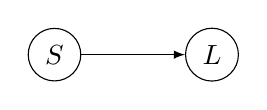
\begin{tikzpicture}[-latex]
\path (0,0) node[draw,circle] (S) {$\RV{S}$}
++(2,0) node[draw,circle] (L) {$\RV{L}$};
\draw (S) -- (L);
\end{tikzpicture}\label{dia:s_causes_l}
\end{align}

when equipped with the \emph{do-scheme} $f:D\to \mathrm{Do}(S\times L)$ given by
\begin{align}
f = \begin{cases}
	d_0 \mapsto \mathrm{do}(\RV{S}=0)\\
	d_1\mapsto \mathrm{do}(\RV{S}=1)
\end{cases}\label{eq:swl_do_scheme}
\end{align}

Once again, the example was setup to suggest this interpretation. I also belive that in the controllable case, veterans of the CBN approach are likely to agree that
\begin{enumerate}
 \item The DAG \ref{dia:s_causes_l} is an appropriate representation of the causal structure of the switch-light example
 \item The two options available do indeed correspond to $do(\RV{S}=0)$ and $do(\RV{S}=1)$; in other words, the do-scheme \ref{eq:swl_do_scheme} is appropriate. I give the informal version here as formal do-schemes aren't a component of the normal DAG approach, but identification of actions available with $do()$ statements is
 \end{enumerate}

This second approach to drawing a causal graph becomes more complicated if we suppose that there are two ways to turn the light on and only one way to turn it off. In this case there is no do-scheme on diagram \ref{dia:s_causes_l} that yields the inequality \ref{eq:three_decisions} as the sole constraint on the results of mixtures of $d_1$ and $d_2$. This is true even if we allow:
\begin{itemize}
	\item Compound $do(..)$ statements like $do(\RV{S}=1,\RV{L}=0)$
	\item The passive $do()$ statement that yields the same distribution over $\RV{S}$ and $\RV{L}$ as was observed
	\item Conditional $do(..)$ operations; e.g. define $g:\{0,1\}\to \{0,1\}$ and let $do(\RV{S}=1,\RV{L}=g(\RV{S}))$ be defined as the operation that sets $\RV{S}=1$ and $\RV{L}=\RV{S}$ 
	\item Stochastic do-schemes e.g. $f(d_0) = 0.25(\delta_{do(\RV{S}=1)} + \delta_{do(\RV{S}=1,\RV{L}=0)} + \delta_{do()} + \delta_{do(\RV{S}=1,\RV{L}=g(\RV{S}))})$
\end{itemize}
In fact this is easy to see: holding observations fixed, the causal theory for three decisions permits any consequence map satisfying \ref{eq:three_decisions}, while fixing any do-scheme on \ref{dia:s_causes_l} will yield a unique consequence map. The situation may be resolved by allowing for observation-dependent uncertainty over do-schemes, but a do scheme with observation-dependent uncertainty can represent any causal theory independent of the graph on which it is defined (this follows from the fact that any consequence map can be represented as a map from actions to mixtures of compound do-statements on every random variable).

It seems reasonable to me to conclude in light of this that diagram \ref{dia:s_causes_l} is not an appropriate diagram for the case of three actions. This is already an interesting result - the notion that diagram \ref{dia:s_causes_l} ``correctly represents the causal relationships of the problem'' can hold when $|D|=2$ but not when $|D|=3$, and the nature of the set $D$ of available actions is rarely given any thought at all in the field of causal graphical models. In defense of the potential outcomes crowd, at least they recognise that this is an assumption that they have to make: 

\begin{quote}
 SUTVA [...] assumes that there are no hidden versions of treatments; no matter how unit i received treatment 1, the outcome that would be observed would be Y i (1) and similarly for treatment 0 \citep{rubin_causal_2005}
\end{quote}


What kind of graph \emph{can} we use when $|D|>=3$?